\hspace{-1cm}
	\begin{tabular}{p{4cm}p{10cm}}
		\hline
		Title & tourism app \\
		\hline
		Date & 16th April 2019 \\
		\hline
		Scene & 1 of 4 \\
		\hline
		Description & This is the landing page \\
		\hline
		Links From Scenes & N/A \\
		\hline
		Links To Scenes & Scene 2 \\
		\hline
		\multicolumn{2}{c}{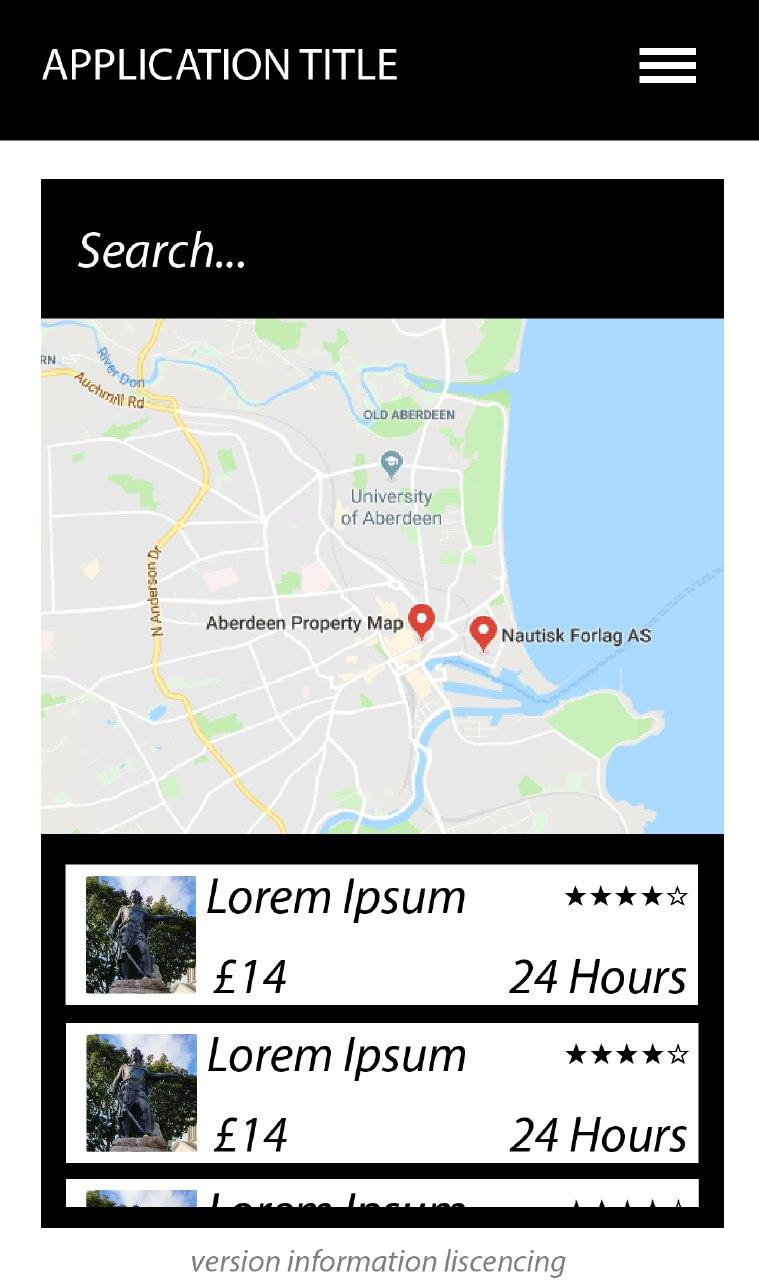
\includegraphics[width=0.5\linewidth]{images/screen0.jpg}} \\
		\hline
		Background & Standard phone background \\
		\hline
		Colour Scehemes Used & Default to black and white but would import from the system theme so users feel immersed \\
		\hline
		Text Attributes & Again, follows system theme (usually a sans-serif font). \\
		\hline
		Audio Files & N/A \\
		\hline
		Video Files & N/A \\
		\hline
		Stills Files & N/A \\
		\hline
		Animations / Movie Clips & N/A \\
		\hline
		\multicolumn{2}{c}{Interface Components (buttons, widgets)} \\
		\hline
		\multicolumn{2}{p{14cm}}{The primary screen of the app shows the hamburger menu in the top right of the screen, with the map of the local area in the centre. Above this lies the search box where a user can search for a particular location if they know the name. In addition, the top locations in the area that the user can tap on to get more information.} \\
		\hline
	\end{tabular}
